\documentclass{article}
\usepackage{graphicx}
\begin{document}

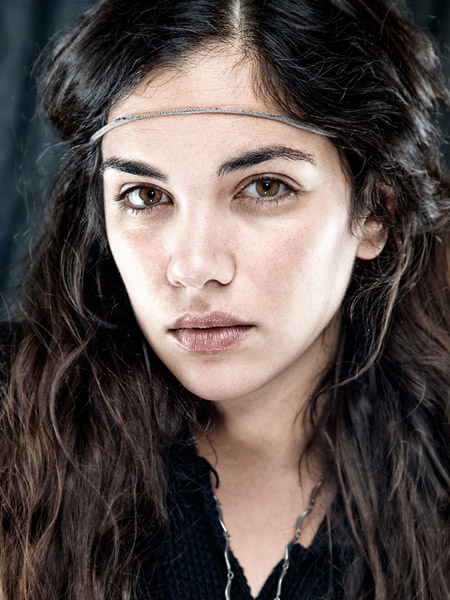
\includegraphics[width=5cm,scale=0.5]{./images/amato}
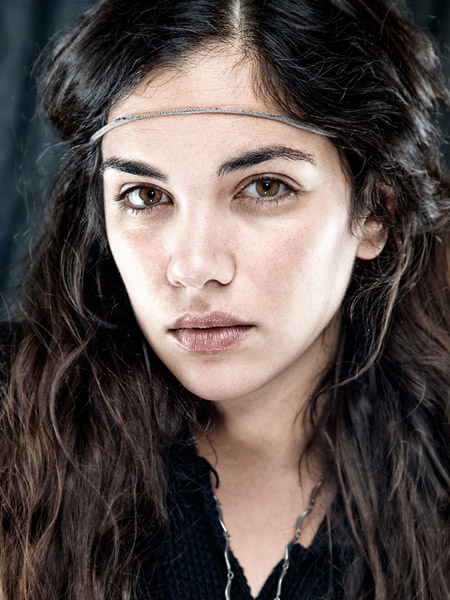
\includegraphics[scale=0.5,scale=0.2]{./images/amato}
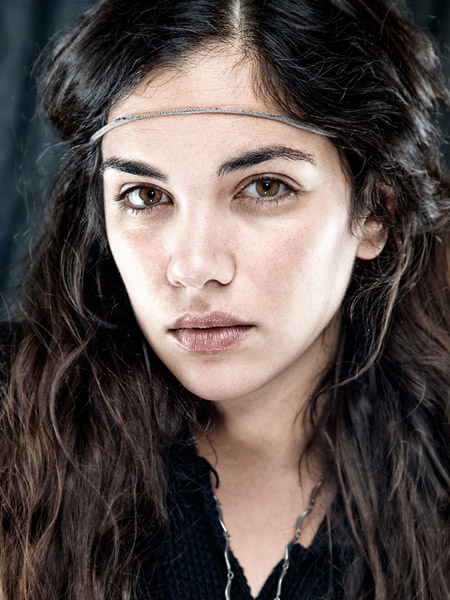
\includegraphics[scale=0.2,scale=0.5,angle=10]{./images/amato}
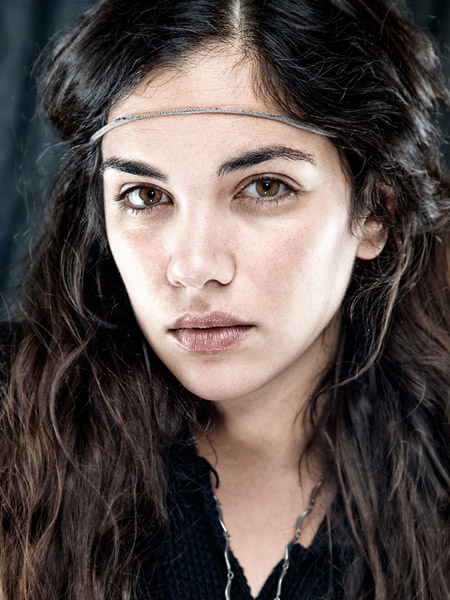
\includegraphics[scale=0.2,scale=0.5,angle=0]{./images/amato}
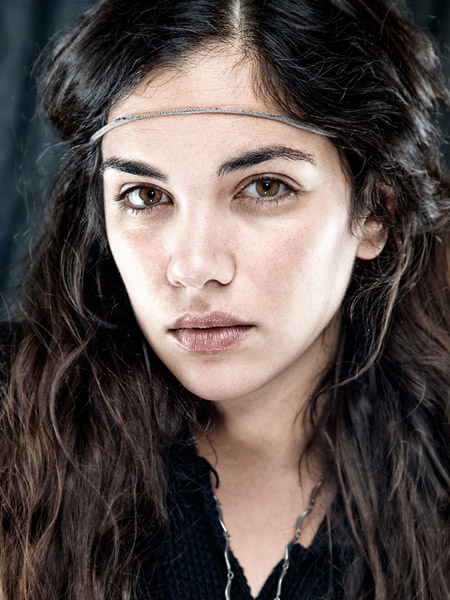
\includegraphics[scale=0.2,angle=-45,angle=-45]{./images/amato}


\def\tokentwo{}
\futurelet\tokenone\tokentwo         
\tt\meaning\tokenone  

\makeatletter
\def\:{\let\@sptoken= } \: % this makes \@sptoken a space token 

\: asd
\meaning\:
\makeatother
\end{document}
Keys with values are cumulative see http://tex.stackexchange.com/questions/195852/rescaling-many-images-which-are-scaled-with-includegraphics/195854?noredirect=1#comment453540_195854

includegraphics keys don't overight they are cumulative and read left to right, mainly so that [height=1cm,angle=90] makes something 1cm wide but [angle=90,height=1cm] makes something 1cm high the fact that you can use two scale is an artifact of the implementation (and not something I've done before this answer I suspect
